\section{Scenario 1}\label{sec:scenario1}
% The purpose of this scenario is to simulate 4 controllers in order to compare them using the map in Figure \ref{fig:s1_map}. 

% \begin{figure}[H]
% 	\hfill
% 	\subfigure[UAS Map Positioning]{\includegraphics[scale=0.33]{figures/s1_p_map.png}}
% 	\hfill
% 	\subfigure[LOS and Distance]{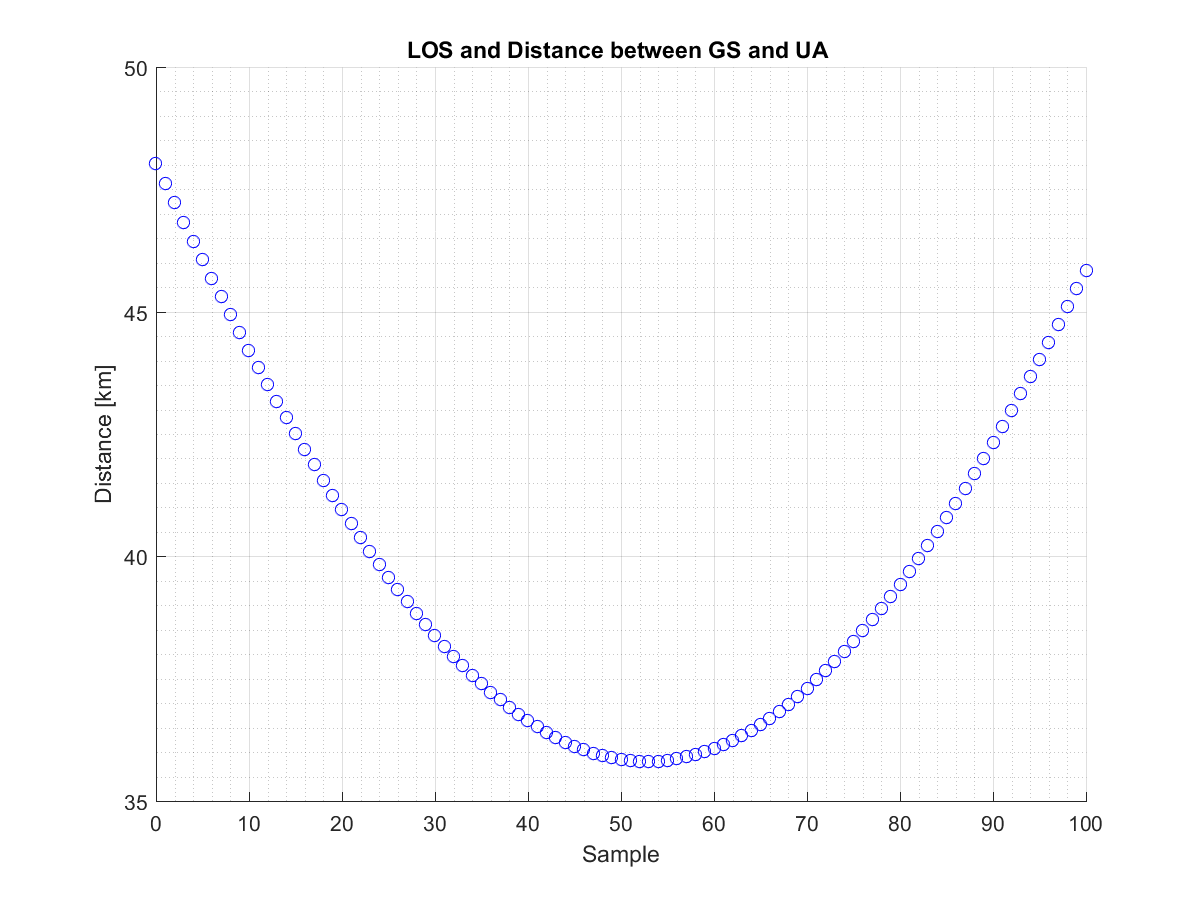
\includegraphics[scale=0.33]{figures/s1_los.png}}
% 	\hfill
% 	\caption{Mountain Scenario}
% 	\label{fig:s1_map}
% \end{figure}

% \subsection{UA}
% In Figure \ref{fig:s1_ua} the angle tracking of the UA antenna can be seen.

% \begin{figure}[H]
% 	\hfill
% 	\subfigure[UAS Map Positioning]{\includegraphics[scale=0.33]{figures/scenario_1_map.png}}
% 	\hfill
% 	\subfigure[LOS and Distance]{\includegraphics[scale=0.33]{figures/scenario_1_los.png}}
% 	\hfill
% 	\caption{Mountain Scenario}
% 	\label{fig:s1_map}
% \end{figure}

% \subsection{GS}
% In Figure \ref{fig:s2_gs} the angle tracking of the GS antenna can be seen.

% \begin{figure}[H]
% \hfill
% \subfigure[UAS Map Positioning]{\includegraphics[scale=0.33]{figures/scenario_1_map.png}}
% \hfill
% \subfigure[LOS and Distance]{\includegraphics[scale=0.33]{figures/scenario_1_los.png}}
% \hfill
% \caption{Mountain Scenario}
% \label{fig:s1_map}
% \end{figure}

% \subsection{Power}
% In Figure \ref{fig:s2_power} the power at the receiver antenna of the GS antenna can be seen.

% \begin{figure}[H]
% \hfill
% \subfigure[UAS Map Positioning]{\includegraphics[scale=0.33]{figures/scenario_1_map.png}}
% \hfill
% \subfigure[LOS and Distance]{\includegraphics[scale=0.33]{figures/scenario_1_los.png}}
% \hfill
% \caption{Mountain Scenario}
% \label{fig:s1_map}
% \end{figure}
